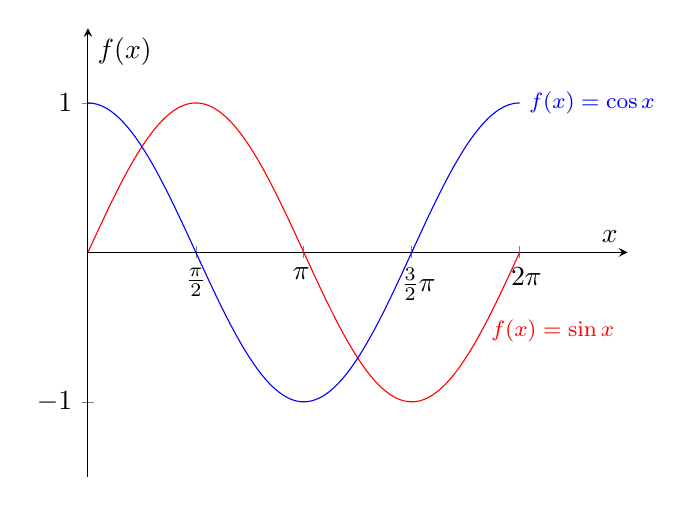
\begin{tikzpicture}
    \begin{axis}[
     clip=false,
     xmin=0,xmax=2.5*pi,
     xlabel= $x$,
     ylabel=$f(x)$,
     ymin=-1.5,ymax=1.5,
     axis lines=middle,
     %axis x line=middle,
     %axis y line=left,
     %axis x line=middle,
     xtick={0,1.57,3.14,4.71,6.28},
     xticklabels={$0$, $\frac{\pi}{2}$,$\pi\,$,$\,\,\,\frac{3}{2}\pi$,$\,\,\,2\pi$},
     %xticklabel style={anchor=north west}
     ]
      \addplot[domain=0:2*pi,samples=200,red]{sin(deg(x))}
                                node[right,pos=0.9,font=\footnotesize]{$f(x)=\sin x$};
      \addplot[domain=0:2*pi,samples=200,blue]{cos(deg(x))}
                                node[right,pos=1,font=\footnotesize]{$f(x)=\cos x$};
    \end{axis}
\end{tikzpicture}
